\documentclass[a1paper]{tikzposter}

\usetheme{Steph}

% Packages
\usepackage[T1]{fontenc}
\usepackage[utf8]{inputenc}
\usepackage{natbib,mdframed,amsmath,calc,graphicx,amssymb,relsize,multirow,rotating,bm,url,multicol,array,subfigure,eurosym}
\usepackage{tikz}
\usetikzlibrary{arrows,patterns, calc, arrows.meta}
\tikzset{>={Latex[width=3mm,length=5mm]}}

\renewcommand{\rmdefault}{phv}
\renewcommand{\sfdefault}{phv} 
\renewcommand{\labelitemi}{$\bullet$}

\newcommand{\compresslist}{
    \setlength{\itemsep}{1pt}
	\setlength{\parskip}{0pt}
	\setlength{\parsep}{0pt}
}

\definecolor{IGNVert}{RGB}{163, 210,  11}
\definecolor{IGNGris}{RGB}{159, 164, 168}
\definecolor{IGNGrisFonce}{RGB}{101, 105, 110}



\title{Conceptualising a co-operative building evolution dashboard on city regions over the past decades for densification studies}
\author{Bénédicte Bucher$^{1}$, Mouhamadou Ndim$^{1}$, Ana-Maria Raimond$^{1}$, Juste Raimbault$^{1}$, Julien Perret$^{1}$, Sebastian Dembski$^{2}$, Mathias Jehling$^{3}$}
\institute{$^{1}$ LASTIG, Univ. Gustave Eiffel, IGN-ENSG\\
$^{2}$ University of Liverpool\\
$^{3}$ Leibniz Institute of Ecological Urban and Regional Development
}
\titlegraphic{}

% Layout of title and logos, some other possible logos are available in images folder
% Don't hesitate to modify the positions if it doesn't suit you
\makeatletter
\renewcommand\TP@maketitle{
    \vspace*{-8cm}
    
    \hspace{.2\textwidth}
    
	\begin{tabular}{lcl}
	    %logo box 1
    	\begin{minipage}[b][.15\textheight][b]{.1\textwidth}

            \vspace{-3cm}
        	
\includegraphics[width=\linewidth]{./figures/LOGO_IGN}\\
            
             \vspace{1cm}
            
            
\includegraphics[width=\linewidth]{./figures/lastig}

            
    	\end{minipage}
    	&
    	%title box
    	\begin{minipage}[b][.2\textheight][b]{.75\textwidth}
    		\centering
    		\color{titlefgcolor}
      
            
    		{\bfseries \LARGE \sc Conceptualising a co-operative building evolution\par}
    		
    		{\bfseries \LARGE \sc dashboard on city regions over the past decades for densification studies \par}
    		\vspace*{1em}
    		{\Large \@author \par}
    		\vspace*{0.5em}
    		{\large \@institute}
    		
    	\end{minipage}
    	&
    	%logo box 2
    	\begin{minipage}[b][.15\textheight][b]{.1\textwidth}

                \vfill
     
            	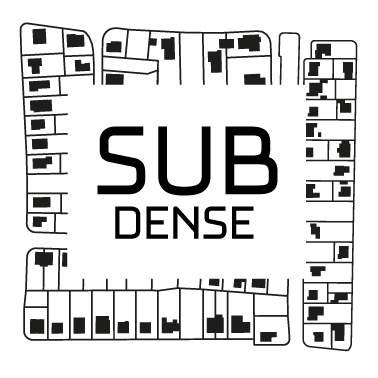
\includegraphics[width=1\textwidth]{./figures/subdense_Logo}

                \vfill
                \vfill
             
    	\end{minipage}
	\end{tabular}
}
\makeatother

%%%%%%%%%%%%%%%%%%%%%%%%%%%%%%%%%%%%%%%%%%%%%%%%%%%%%%%%%%%%%%%%%%%%%%%%%%%%%%%%
% Multicol Settings
%%%%%%%%%%%%%%%%%%%%%%%%%%%%%%%%%%%%%%%%%%%%%%%%%%%%%%%%%%%%%%%%%%%%%%%%%%%%%%%%
\setlength{\columnsep}{1.5em}
\setlength{\columnseprule}{0mm}

%%%%%%%%%%%%%%%%%%%%%%%%%%%%%%%%%%%%%%%%%%%%%%%%%%%%%%%%%%%%%%%%%%%%%%%%%%%%%%%%
% Save space in lists. Use this after the opening of the list
%%%%%%%%%%%%%%%%%%%%%%%%%%%%%%%%%%%%%%%%%%%%%%%%%%%%%%%%%%%%%%%%%%%%%%%%%%%%%%%%


% To remove the "latex tikz poster" at the bottom right corner
\tikzposterlatexaffectionproofoff

\begin{document}
	% Title block with title, author, logo, etc.
	\maketitle
	
%------------------------------------------------------
%----------------LINE 1--------------------------------
%------------------------------------------------------
% block alone on its line so you don't have to specify the columns environment


		%==============================================
		\block[titlewidthscale=0.5]{Context: The SubDense project}{

            
			\begin{itemize}
				\item Suburban densification can yield more \emph{sustainable cities} while avoiding over-densification in centres.
				\item Coexistence of \emph{multiple rationalities} for involved stakeholders imply considerable \emph{planning challenges}.
			\end{itemize}

                 \bigskip

                The \textbf{SubDense} European project aims at better understanding how diverse \textbf{strategies of land policy} shape suburban densification across different \textbf{planning systems} (France, Germany, UK).
   
		}
		%==============================================

  

	
	%==============================================
	\block[titlewidthscale=0.5]{Collaborative dashboard}{
		\parbox{0.5\textwidth}{
			\begin{mdframed}
                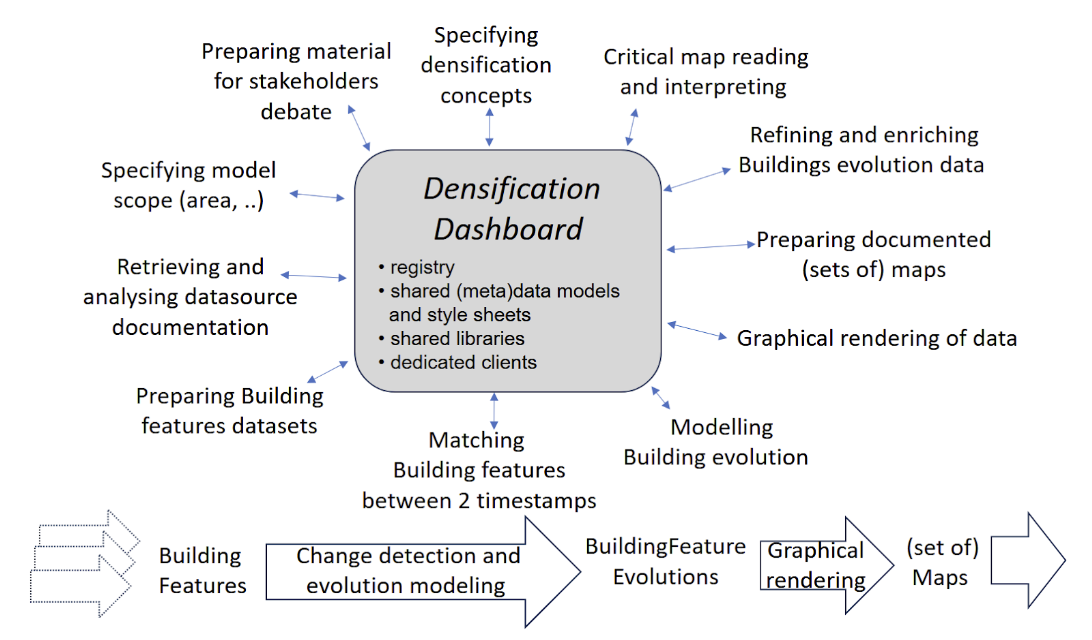
\includegraphics[width=\linewidth]{figures/dashboard.png}
		      \end{mdframed}
            }
         \hspace{1cm}
		\parbox{0.3\textwidth}{
            
            $\rightarrow$ A \textbf{collaborative dashboard} as a medium to \textbf{facilitate collaboration} between partners, \textbf{share methods, data and metadata} \cite{bucher2020conciliating}, and ensure reproducibility 

            
   
		}
		%==============================================
	}


        \block[titlewidthscale=0.5]{Architecture and implementation}{

            \parbox{0.5\textwidth}{
			\begin{mdframed}
                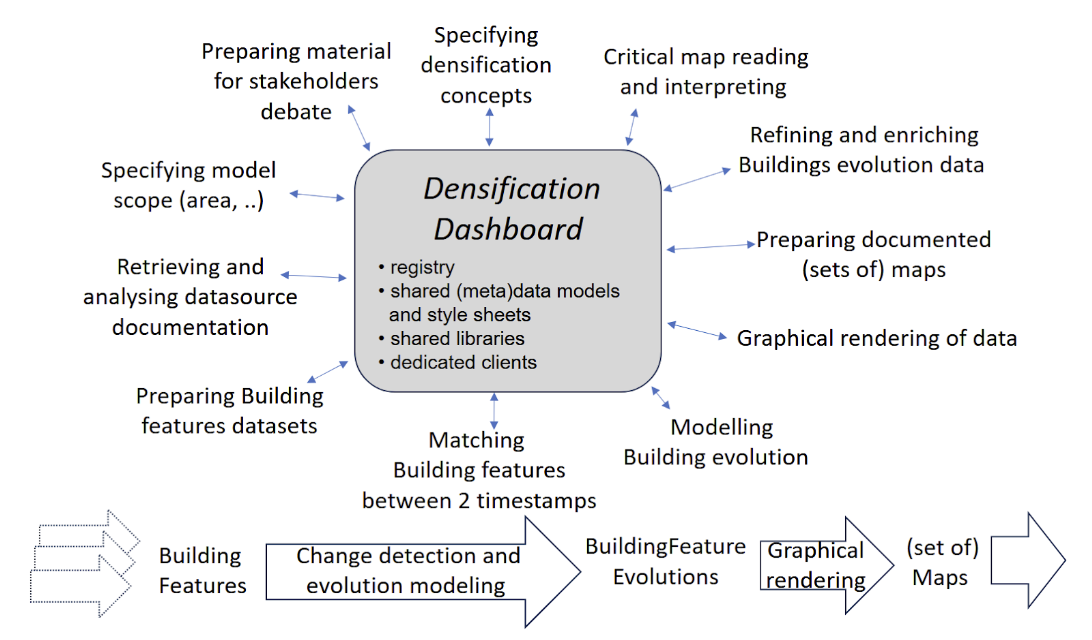
\includegraphics[width=\linewidth]{figures/dashboard.png}
		      \end{mdframed}
            }
         
			$\rightarrow$ The \textbf{git-based architecture} for the core dashboard ensures tractability, full history, reproducibility, flexibility, and collaboration through branching, shared remote repository (\url{https://github.com/subdense}).

            \bigskip
    
            $\rightarrow$ Clients implement interactions with the core and functionalities needed by partners for data analysis and integration (running change detection algorithms, adding data, exploring results and maps, \ldots).


           % $\rightarrow$ An iterative process to produce \textbf{user stories}, finally leading to some specifications for the core architecture and functionalities of clients.


        }

         
%------------------------------------------------------
%----------------LINE 4--------------------------------
%------------------------------------------------------

	\begin{columns}
		%In this block you can specify possible improvment or any extra information
		\column{0.4}
		%==============================================
		\block[titlewidthscale=0.65]{Future work}{
			\begin{itemize}
				\item \emph{heterogeneous data integration} \cite{bucher2021towards}, to couple densification analysis with socio-economic data;
                \item develop and explore \emph{simulation models} for the impact of policies on densification processes, parametrise these models with the qualitative data obtained through interviews during the project.
			\end{itemize}
		}
		
	
		
		\column{0.6}
		%==============================================
		% bibliography managed with natbib
		\block[titlewidthscale=0.3,bodyoffsety=1.8cm,titleoffsety=.1cm]{References}{
			% This command is to prevent the printing of a second "références" in text and to delete white space between block title and bibliography
			\renewcommand\refname{\vskip -2cm}
			% Bibliography input. 
			%Refrences should be added directly to the Biblio.bib file. Refrences should in bibTex Format. Every Reference cited in the poster will be automatically added.
            \footnotesize
   
			\bibliography{Biblio}
			% Plain style so that cited articles appear as number in the poster and are only fully displayed here
			\bibliographystyle{plain}
		}
	    %==============================================	
	\end{columns}
	
\node [above right,outer sep=20pt,minimum width=\textwidth,align=center,draw=none,fill=none, text = IGNGrisFonce] at (bottomleft) {\centering \huge \bf AGILE 2024};

\end{document}

\endinput


\begin{columns}
		
		\column{0.5}
		%==============================================
		\block[titlewidthscale=0.7]{Data expertise and analysis}{

            \begin{center}
            \includegraphics[width=0.5\linewidth]{figures/building_evolution.png}
            \hspace{2cm}
            \includegraphics[width=0.25\linewidth]{figures/compar_bdtopo.png}
            \end{center}
            
            \bigskip

            $\rightarrow$ how to share analysis and methods for reproduction on other case studies (\textit{Left figure}: example of change analysis)

            \bigskip
            
            % how to integrate this knowledge on data specification into the dashboard so that it is discoverable and reusable by partners?

            $\rightarrow$ how to integrate knowledge on data specification (\textit{Right figure}: change in specifications of BDTopo 2020-2022) so that partners' analysis are not biased?
   
		}
		
		\column{0.5}
		%==============================================
		\block[titlewidthscale=0.9]{Matching algorithms for change detection}{

            \parbox{0.75\linewidth}{
              \includegraphics[width=\linewidth]{figures/matching}
		      }
            \hspace{0.5cm}
            \parbox{0.2\linewidth}{
			    \textbf{Typology of changes}

                \bigskip

                {\textcolor{green!50!black}{1:1 stability}}

                {\textcolor{blue}{1:0 destruction}}

                {\textcolor{magenta}{0:1 construction}}
		      }
  
            \vspace{1.6cm}

            $\rightarrow$ Benchmark of polygon matching algorithms \cite{olteanu2015knowledge}, to provide tools for building change detection

            
   
		}
		%==============================================
		
		
	\end{columns}


% Third column on first line
		\column{0.36}% Width set relative to text width
		%==============================================
		\block[titlewidthscale=0.7]{Work packages}{

           
			\begin{itemize}
				\item \textbf{WP1:} Which data, information infrastructures and approaches enable a comparative spatial analysis of suburban densification and allow for an integration of stakeholders' interests and agency?
    
    $\rightarrow$ \textbf{main LASTIG contribution: } data integration, collaboration in data analysis, geosimulation.
				\item \textbf{WP2:} How can stakeholders' interests and agency be explained in relation to land policies for suburban densification?
                \item \textbf{WP3:} How do land policies respond to the interests and agency of stakeholders in an effective and efficient way?
			\end{itemize}
		}


\column{0.25}
		%==============================================
		\block[titlewidthscale=0.5]{Project details}{
            
            \vspace{1cm}
			
            \begin{itemize}
				\item January 2023 -- December 2025
				\item \textit{Open Research Area for the Social Sciences} European grant: 1M\euro
				\item 4 partner institutions: TU Dortmund, IOER, University of Liverpool, IGN
                \item 8 permanent researchers, 5 short-term contracts working full time
			\end{itemize}

            \vspace{0.3cm}
   
		}



% Template


			\vspace{.5cm}
			
			%This block contain example of Tikz
			
			\centering
			
			\begin{tikzpicture}[scale=2]
			\draw[-latex] (0,0) -- (0,3.2);
			\draw[-latex] (0,0) -- (5.2,0);
			\node at (-0.2,1.5) {$\theta$};
			\node at (2.5,-0.2) {$\mathit{t}$};
			
			\node at (0.2,0) {$\bullet$};
			\node at (0.4,0.8) {$\bullet$};
			\node at (0.6,1.6) {$\bullet$};
			\node at (0.8,2.4) {$\bullet$};
			\node at (1.8,0.4) {$\bullet$};
			\node at (2,1.2) {\textcolor{red!60!black}{$\bullet$}};
			\node at (2.2,2) {$\bullet$};
			\node at (2.4,2.8) {$\bullet$};
			\node at (3.4,0) {$\bullet$};
			\node at (3.6,0.8) {$\bullet$};
			\node at (3.8,1.6) {$\bullet$};
			\node at (4,2.4) {$\bullet$};
			
			\draw[->,red!60!black] (2,1.2) -- (0.4,0.8);
			\draw[->,red!60!black] (2,1.2) -- (0.6,1.6);
			\draw[->,red!60!black] (2,1.2) -- (1.8,0.4);
			\draw[->,red!60!black] (2,1.2) -- (2.2,2);
			\draw[->,red!60!black] (2,1.2) -- (3.6,0.8);
			\draw[->,red!60!black] (2,1.2) -- (3.8,1.6);
			\end{tikzpicture}
			
			Exemple de Tikz 

			\vspace{.5cm}
			


